\documentclass[parskip=full]{scrartcl}
\usepackage[utf8]{inputenc} % use utf8 file encoding for TeX sources
\usepackage[T1]{fontenc}    % avoid garbled Unicode text in pdf
\usepackage[german]{babel}  % german hyphenation, quotes, etc
\usepackage{hyperref}       % detailed hyperlink/pdf configuration
\hypersetup{                % ‘texdoc hyperref‘ for options
pdftitle={SWT1: Lastenheftvorlage},%
bookmarks=true,%
}
\usepackage{graphicx}       % provides commands for including figures
\usepackage{csquotes}       % provides \enquote{} macro for "quotes"
\usepackage[nonumberlist]{glossaries}     % provides glossary commands
\usepackage{enumitem}

\makenoidxglossaries
%
% % Glossareinträge
%
\newglossaryentry{Smartphone}
{
	name=Smartphone,
	plural=Smartphones,
	description={Mobiltelefon, welches erweiterte Funktionen wie GPS und die Installation von Apps zur Verfügung stellt.},
}

\newglossaryentry{Kunde}
{
	name=Kunde,
	plural=Kunden,
	description={(Zahlende) Nutzer der App iMage.}
}

\newglossaryentry{Applikation}
{
	name=Applikation,
	plural=Applikationen,
	description={Anwendung, welche z.B. auf einem Smartphone installiert werden kann.}
}

\newglossaryentry{HDR Bild}
{
	name=HDR Bild,
	plural=HDR Bilder,
	description={HDR steht für High Dynamic Range Bild. Grafik, welche hohe Helligkeitsstufen detailreich wiedergibt.}
}

\newglossaryentry{soziales Netzwerk}
{
	name=soziales Netzwerk,
	plural=soziale Netzwerke,
	description={Seite im Internet, welche den Informationsaustausch und Kontakt zwischen Menschen fördert. Beispiele hierfür sind Facezine und Instagrim.}
}

\title{SWT1: Lastenheft iMage}
\author{Daniel Vollmer, 2219041}

\begin{document}

\maketitle

%
% % Hier beginnt die Gliederung des Lastenhefts
%
\section{Zielbestimmung}
iMage ist eine \gls{Applikation} (App) der Firma Pear Corp. Diese soll in der Lage sein \glspl{HDR Bild} auf Grundlage von vom \glspl{Kunde} ausgewählten Bildern zu erstellen. Zur Speicherung muss der Kunde entweder eine Einmalzahlung tätigen oder ein Monatsabonnement abschließen. Der Kunde soll außerdem in der Lage sein erstellte Bilder direkt auf sozialen Medien zu teilen.

\section{Produkteinsatz}
Das Produkt dient dem Kunden dazu mit einem mobilen Endgerät \glspl{HDR Bild} zu erzeugen, speichern und teilen in sozialen Netzwerken.

Zielgruppe: Alle \glspl{Kunde} mit einem mobilen Endgerät, welche sich für die Erstellung von \glspl{HDR Bild}n interessieren.

Plattform: Smartphone (Android und iOS für optimale Kundenabdeckung. Für optimale Performance der Anwendung soll ein Smartphone der mittleren Preisklasse bereits ausreichen.)

\section{Funktionale Anforderungen}
\begin{itemize}[nosep]
\item[FA10] Bereitstellung einer Übersicht über das Nutzerkonto und der zuletzt erstellten \glspl{HDR Bild} auf der Startseite.
\item[FA20] Anzeigen einer Vorschau beim Klick auf ein bereits erstelltes \glspl{HDR Bild}, sowie die Anzeige eines "Schließen" Buttons zum beenden der Vorschau und eines "Teilen" Buttons zum hochladen in \glspl{soziales Netzwerk}.
\item[FA30] Ein Button "Neues HDR-Bild" auf der Startseite. Durch diesen soll der \gls{Kunde} zu einer Übersicht seiner auf dem \gls{Smartphone} gespeicherten Bilder gelangen. Nach Auswahl dreier Bilder und einer Bestätigung auf den Button "HDR-Bild" soll die Erzeugung eines neuen \gls{HDR Bild}es auf Grundlage der ausgewählten Bilder eingeleitet werden.
\item[FA40] Erzeugung eines \gls{HDR Bild}es. Dazu werden die benötigten Daten auf den Pear-Corp-Zentralserver hochgeladen. 
\item[FA50] Erzeugte Bilder vom Pear-Corp-Zentralserver über den Button "HDR-Bild abholen".
\item[FA60] Einrichtung eines Monatsabonnements oder einer Einmalzahlung des \glspl{Kunde}, um die erstellten \glspl{HDR Bild} beim Klick auf den "HDR-Bild abholen" Button zu erhalten. Hat der \gls{Kunde} bereits ein Monatsabonnement abgeschlossen, so entfällt diese Einrichtung und es wird sofort der "HDR-Bild jetzt speichern" Button angezeigt, durch welchen das Bild gespeichert wird.
\item[FA70] Dauerhafte Speicherung aller Bilder zur Analyse der Nutzererfahrng auf dem Pear-Corp-zentralserver.
\end{itemize}

\section{Produktdaten}
\begin{itemize}[nosep]
\item[PD10] Es sind relevante Daten über die Kunden zu speichern.
\item[PD20] Die Zahlungsinformationen und Zahlungsart des Kunden sind zu speichern.
\item[PD30] Es sind alle Bilder (Eingabe- und Ergebnisbilder) des Kunden zu speichern.
\end{itemize}

\section{Nichtfunktionale Anforderungen}
\begin{itemize}[nosep]
\item[NF10] Die Übersicht aller Bilder auf dem \gls{Smartphone} des \glspl{Kunde} (Funktion /FA30/) soll in Echtzeit bis zu 100 Bilder aneigen können.
\item[NF20] Mindestens 1000 \glspl{Kunde} müssen gleichzeitig mit dem Pear-Corp-Zentralserver kommunizieren können.
\item[NF30] Dier Erzeugung eines \gls{HDR Bild}es darf nicht länger als sieben Sekunden dauern.
\end{itemize} 

\section{Systemmodelle}

\subsection{Szenarien}

\subsection{Anwendungsfälle}
\subsubsection{Seminarorganisation}
\begin{center}
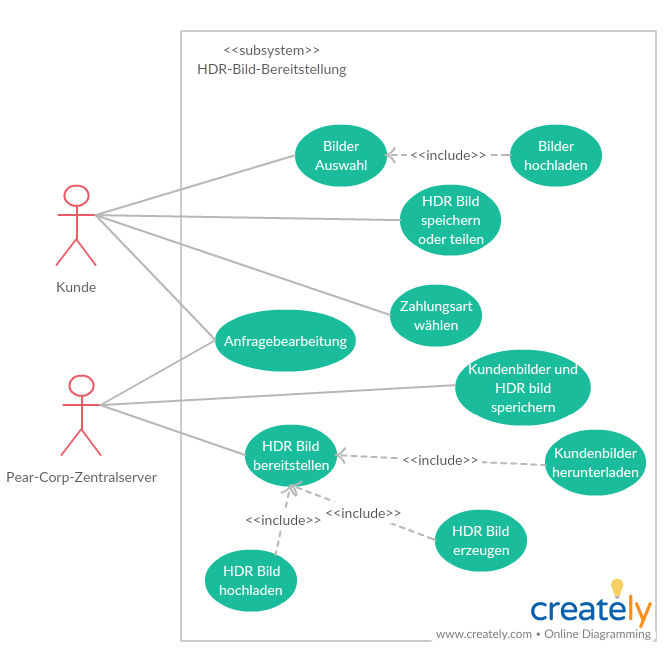
\includegraphics[width=0.8\textwidth]{Szenario1.jpg}
\end{center}

Akteure: Kunde, Pear-Corp-Zentralserver.

Anwendungsfälle: Bilder Auswahl, Bilder hochladen, \gls{HDR Bild} speichern oder teilen, Zahlungsart wählen, Anfragebearbeitung, Kundenbilder und \gls{HDR Bild} speichern, \gls{HDR Bild} bereitstellen, \gls{HDR Bild} hochladen, \gls{HDR Bild} erzeugen, Kundenbilder herunterladen.

Textuelle Beschreibung: (folgt)



%
% % Automatisch generiertes Glossar (Latex zwei mal ausführen um Glossar anzuzeigen)
%
%\glsaddall % das sorgt dafür, dass alles Glossareinträge gedruckt werden, nicht nur die verwendeten. Das sollte nicht nötig sein!
\printnoidxglossaries
Siehe \url{https://en.wikibooks.org/wiki/LaTeX/Glossary}.




\end{document}
